\section{На салфетке}

\begin{enumerate}
\itA Укажите, как нарисовать «одним росчерком пера», то есть не отрывая ручки от бумаги и не проходя по одной линии дважды, (а) олимпийские кольца (б) «наклонный квадрат» со стороной 4 (см.\,рисунок\,5).

\centerline{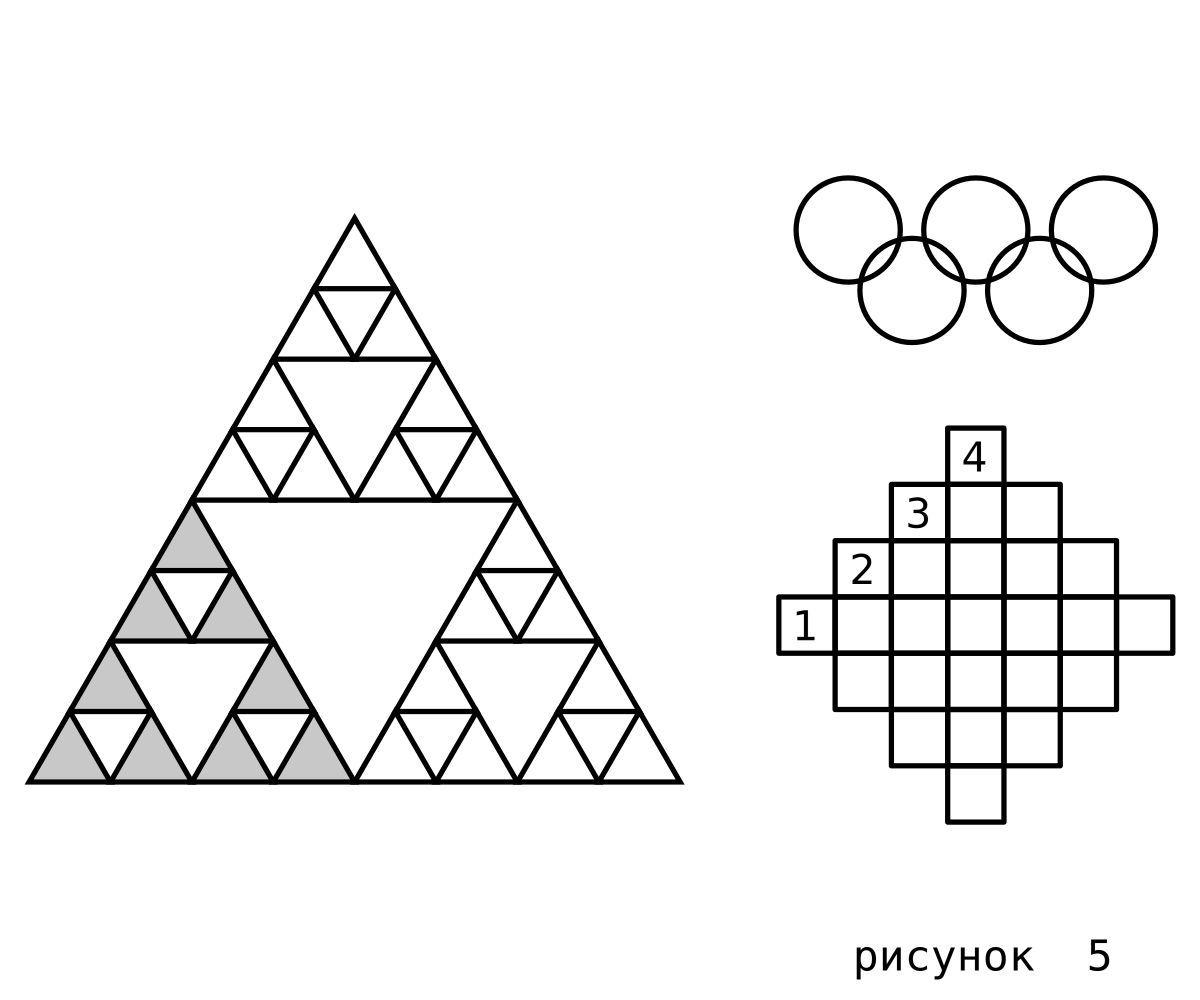
\includegraphics[width=5.5cm]{images/serpinsky}}

\itB Треугольник Серпинского степени 1 — это просто треугольник. Чтобы получить треугольник Серпинского степени $n+1$, нужно поставить «друг на друга» три треугольника Серпинского степени $n$. На рисунке 5 изображён треугольник Серпинского степени 4, а цветом выделен треугольник Серпинского степени 3. Посчитайте, сколько узлов (точек, где пересекаются два и более непараллельных отрезка) в треугольнике Серпинского степени $n$. Посчитайте также, сколько отрезков длины 1 составляют «наклонный квадрат» со стороной $n$.

\itC Укажите, как нарисовать одним росчерком пера треугольник Серпинского степени 4, изображённый на рисунке {\tt T-S}.
\end{enumerate}